\documentclass[10pt]{article}
\usepackage[paperwidth=17in,paperheight=11in,margin=0.35in]{geometry}
\usepackage{tikz}
\usepackage{graphicx}
\usepackage[scaled]{helvet}
\renewcommand{\familydefault}{\sfdefault}
\usetikzlibrary{arrows.meta,positioning,fit,calc,backgrounds}
\pagestyle{empty}

\definecolor{ink}{HTML}{1F2937}
\definecolor{muted}{HTML}{4B5563}
\definecolor{interface}{HTML}{2563EB}
\definecolor{interfacebg}{HTML}{EFF6FF}
\definecolor{runtime}{HTML}{0F766E}
\definecolor{runtimebg}{HTML}{ECFDF5}
\definecolor{quail}{HTML}{B45309}
\definecolor{quailbg}{HTML}{FFF7ED}
\definecolor{store}{HTML}{475569}
\definecolor{storebg}{HTML}{F8FAFC}
\definecolor{external}{HTML}{7C3AED}
\definecolor{externalbg}{HTML}{F5F3FF}
\definecolor{state}{HTML}{BE123C}
\definecolor{statebg}{HTML}{FFF1F2}

\newcommand{\nodeTitle}[1]{\textbf{\small #1}}
\newcommand{\code}[1]{{\ttfamily\scriptsize #1}}

\begin{document}
\begin{center}
\resizebox{0.98\linewidth}{!}{%
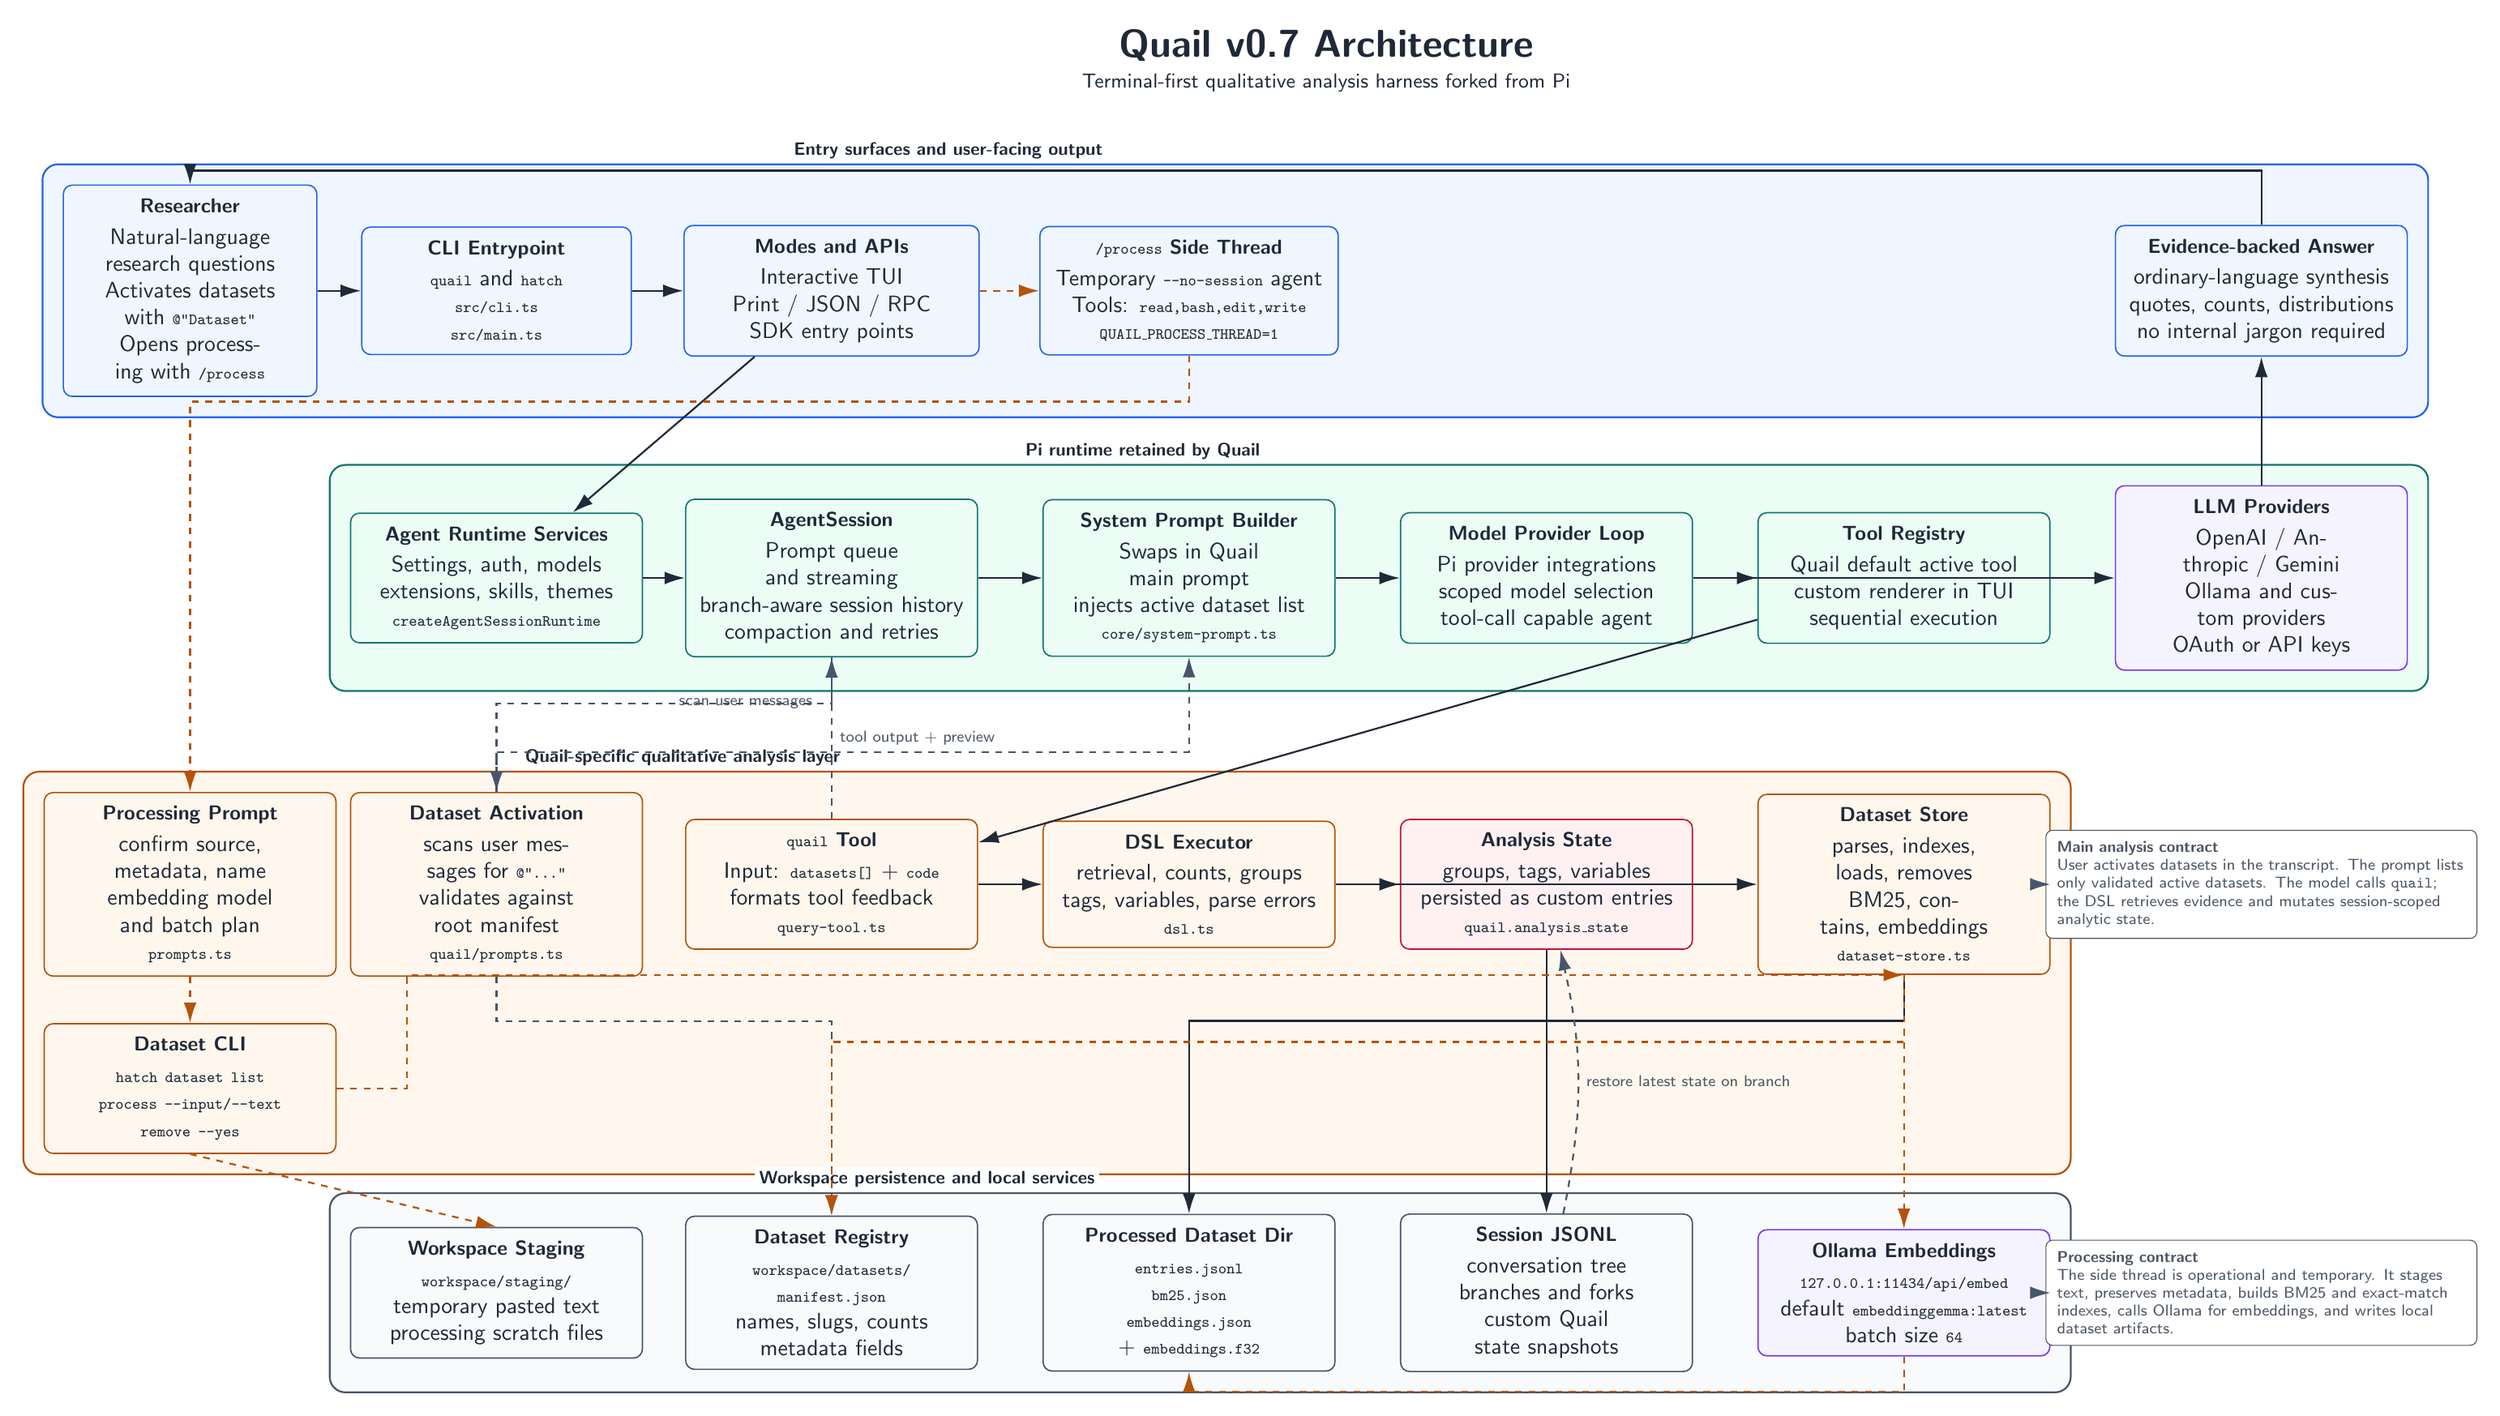
\begin{tikzpicture}[
  node distance=1.0cm,
  font=\sffamily,
  block/.style={
    rectangle,
    rounded corners=4pt,
    draw=ink,
    line width=0.6pt,
    align=center,
    text=ink,
    inner sep=6pt,
    minimum height=1.28cm
  },
  lane/.style={
    rectangle,
    rounded corners=7pt,
    line width=0.8pt,
    inner sep=9pt
  },
  laneLabel/.style={
    font=\bfseries\footnotesize,
    text=ink,
    fill=white,
    inner sep=2pt
  },
  flow/.style={
    -{Latex[length=3.2mm,width=2.0mm]},
    draw=ink,
    line width=0.8pt
  },
  dataflow/.style={
    -{Latex[length=3.2mm,width=2.0mm]},
    draw=store,
    line width=0.8pt,
    dashed
  },
  sideflow/.style={
    -{Latex[length=3.2mm,width=2.0mm]},
    draw=quail,
    line width=0.8pt,
    dashed
  },
  note/.style={
    rectangle,
    rounded corners=3pt,
    draw=muted,
    fill=white,
    align=left,
    text=muted,
    font=\scriptsize,
    inner sep=5pt
  }
]

% Title
\node[align=center, text=ink] (title) at (20,24.1)
  {\textbf{\LARGE Quail v0.7 Architecture}\\[2pt]
  \small Terminal-first qualitative analysis harness forked from Pi};

% Entry surfaces
\node[block, fill=interfacebg, draw=interface, text width=3.55cm] (user) at (2.2,20.5)
  {\nodeTitle{Researcher}\\[2pt]
  Natural-language research questions\\
  Activates datasets with \code{@"Dataset"}\\
  Opens processing with \code{/process}};

\node[block, fill=interfacebg, draw=interface, text width=3.8cm] (cli) at (7.0,20.5)
  {\nodeTitle{CLI Entrypoint}\\[2pt]
  \code{quail} and \code{hatch}\\
  \code{src/cli.ts}\\
  \code{src/main.ts}};

\node[block, fill=interfacebg, draw=interface, text width=4.2cm] (modes) at (12.25,20.5)
  {\nodeTitle{Modes and APIs}\\[2pt]
  Interactive TUI\\
  Print / JSON / RPC\\
  SDK entry points};

\node[block, fill=interfacebg, draw=interface, text width=4.25cm] (processThread) at (17.85,20.5)
  {\nodeTitle{\code{/process} Side Thread}\\[2pt]
  Temporary \code{--no-session} agent\\
  Tools: \code{read,bash,edit,write}\\
  \code{QUAIL\_PROCESS\_THREAD=1}};

% Runtime lane
\node[block, fill=runtimebg, draw=runtime, text width=4.15cm] (runtimeServices) at (7.0,16.0)
  {\nodeTitle{Agent Runtime Services}\\[2pt]
  Settings, auth, models\\
  extensions, skills, themes\\
  \code{createAgentSessionRuntime}};

\node[block, fill=runtimebg, draw=runtime, text width=4.15cm] (agentSession) at (12.25,16.0)
  {\nodeTitle{AgentSession}\\[2pt]
  Prompt queue and streaming\\
  branch-aware session history\\
  compaction and retries};

\node[block, fill=runtimebg, draw=runtime, text width=4.15cm] (systemPrompt) at (17.85,16.0)
  {\nodeTitle{System Prompt Builder}\\[2pt]
  Swaps in Quail main prompt\\
  injects active dataset list\\
  \code{core/system-prompt.ts}};

\node[block, fill=runtimebg, draw=runtime, text width=4.15cm] (modelLoop) at (23.45,16.0)
  {\nodeTitle{Model Provider Loop}\\[2pt]
  Pi provider integrations\\
  scoped model selection\\
  tool-call capable agent};

\node[block, fill=runtimebg, draw=runtime, text width=4.15cm] (toolRegistry) at (29.05,16.0)
  {\nodeTitle{Tool Registry}\\[2pt]
  Quail default active tool\\
  custom renderer in TUI\\
  sequential execution};

% Quail domain lane
\node[block, fill=quailbg, draw=quail, text width=4.15cm] (activation) at (7.0,11.2)
  {\nodeTitle{Dataset Activation}\\[2pt]
  scans user messages for \code{@"..."}\\
  validates against root manifest\\
  \code{quail/prompts.ts}};

\node[block, fill=quailbg, draw=quail, text width=4.15cm] (queryTool) at (12.25,11.2)
  {\nodeTitle{\code{quail} Tool}\\[2pt]
  Input: \code{datasets[]} + \code{code}\\
  formats tool feedback\\
  \code{query-tool.ts}};

\node[block, fill=quailbg, draw=quail, text width=4.15cm] (dsl) at (17.85,11.2)
  {\nodeTitle{DSL Executor}\\[2pt]
  retrieval, counts, groups\\
  tags, variables, parse errors\\
  \code{dsl.ts}};

\node[block, fill=statebg, draw=state, text width=4.15cm] (analysisState) at (23.45,11.2)
  {\nodeTitle{Analysis State}\\[2pt]
  groups, tags, variables\\
  persisted as custom entries\\
  \code{quail.analysis\_state}};

\node[block, fill=quailbg, draw=quail, text width=4.15cm] (datasetStore) at (29.05,11.2)
  {\nodeTitle{Dataset Store}\\[2pt]
  parses, indexes, loads, removes\\
  BM25, contains, embeddings\\
  \code{dataset-store.ts}};

% Processing lane
\node[block, fill=quailbg, draw=quail, text width=4.15cm] (processingPrompt) at (2.2,11.2)
  {\nodeTitle{Processing Prompt}\\[2pt]
  confirm source, metadata, name\\
  embedding model and batch plan\\
  \code{prompts.ts}};

\node[block, fill=quailbg, draw=quail, text width=4.15cm] (datasetCli) at (2.2,8.0)
  {\nodeTitle{Dataset CLI}\\[2pt]
  \code{hatch dataset list}\\
  \code{process --input/--text}\\
  \code{remove --yes}};

% Persistence and external systems
\node[block, fill=storebg, draw=store, text width=4.15cm] (staging) at (7.0,4.8)
  {\nodeTitle{Workspace Staging}\\[2pt]
  \code{workspace/staging/}\\
  temporary pasted text\\
  processing scratch files};

\node[block, fill=storebg, draw=store, text width=4.15cm] (registry) at (12.25,4.8)
  {\nodeTitle{Dataset Registry}\\[2pt]
  \code{workspace/datasets/}\\
  \code{manifest.json}\\
  names, slugs, counts\\
  metadata fields};

\node[block, fill=storebg, draw=store, text width=4.15cm] (datasetFiles) at (17.85,4.8)
  {\nodeTitle{Processed Dataset Dir}\\[2pt]
  \code{entries.jsonl}\\
  \code{bm25.json}\\
  \code{embeddings.json} + \code{embeddings.f32}};

\node[block, fill=storebg, draw=store, text width=4.15cm] (sessions) at (23.45,4.8)
  {\nodeTitle{Session JSONL}\\[2pt]
  conversation tree\\
  branches and forks\\
  custom Quail state snapshots};

\node[block, fill=externalbg, draw=external, text width=4.15cm] (ollama) at (29.05,4.8)
  {\nodeTitle{Ollama Embeddings}\\[2pt]
  \code{127.0.0.1:11434/api/embed}\\
  default \code{embeddinggemma:latest}\\
  batch size \code{64}};

\node[block, fill=externalbg, draw=external, text width=4.15cm] (providers) at (34.65,16.0)
  {\nodeTitle{LLM Providers}\\[2pt]
  OpenAI / Anthropic / Gemini\\
  Ollama and custom providers\\
  OAuth or API keys};

\node[block, fill=interfacebg, draw=interface, text width=4.15cm] (answer) at (34.65,20.5)
  {\nodeTitle{Evidence-backed Answer}\\[2pt]
  ordinary-language synthesis\\
  quotes, counts, distributions\\
  no internal jargon required};

% Background lane labels
\begin{scope}[on background layer]
  \node[lane, fill=interfacebg, draw=interface, fit=(user)(cli)(modes)(processThread)(answer),
    label={[laneLabel]above left:Entry surfaces and user-facing output}] {};
  \node[lane, fill=runtimebg, draw=runtime, fit=(runtimeServices)(agentSession)(systemPrompt)(modelLoop)(toolRegistry)(providers),
    label={[laneLabel]above left:Pi runtime retained by Quail}] {};
  \node[lane, fill=quailbg, draw=quail, fit=(processingPrompt)(activation)(queryTool)(dsl)(analysisState)(datasetStore)(datasetCli),
    label={[laneLabel]above left:Quail-specific qualitative analysis layer}] {};
  \node[lane, fill=storebg, draw=store, fit=(staging)(registry)(datasetFiles)(sessions)(ollama),
    label={[laneLabel]above left:Workspace persistence and local services}] {};
\end{scope}

% Main flow
\draw[flow] (user) -- (cli);
\draw[flow] (cli) -- (modes);
\draw[flow] (modes) -- (runtimeServices);
\draw[flow] (runtimeServices) -- (agentSession);
\draw[flow] (agentSession) -- (systemPrompt);
\draw[flow] (systemPrompt) -- (modelLoop);
\draw[flow] (modelLoop) -- (toolRegistry);
\draw[flow] (toolRegistry) -- (queryTool);
\draw[flow] (queryTool) -- (dsl);
\draw[flow] (dsl) -- (datasetStore);
\draw[flow] (datasetStore.south) -- ++(0,-0.72) -| (datasetFiles.north);
\draw[flow] (dsl) -- (analysisState);
\draw[flow] (analysisState) -- (sessions);
\draw[flow] (modelLoop) -- (providers);
\draw[flow] (providers) -- (answer);
\draw[flow] (answer.north) -- ++(0,0.85) -| (user.north);

% Dataset activation and prompt context
\draw[dataflow] (agentSession.south) -- ++(0,-0.72) -| node[pos=0.24, right, font=\scriptsize, text=muted] {scan user messages} (activation.north);
\draw[dataflow] (activation.south) -- ++(0,-0.7) -| (registry.north);
\draw[dataflow] (activation.north) -- ++(0,0.62) -| (systemPrompt.south);

% Tool results and branch-aware state
\draw[dataflow] (queryTool.north) -- node[right, font=\scriptsize, text=muted] {tool output + preview} (agentSession.south);
\draw[dataflow] (sessions) to[bend right=12] node[right, font=\scriptsize, text=muted] {restore latest state on branch} (analysisState);

% Processing flow
\draw[sideflow] (modes) -- (processThread);
\draw[sideflow] (processThread.south) -- ++(0,-0.72) -| (processingPrompt.north);
\draw[sideflow] (processingPrompt) -- (datasetCli);
\draw[sideflow] (datasetCli.south) -- (staging.north);
\draw[sideflow] (datasetCli.east) -- ++(1.1,0) |- (datasetStore.south);
\draw[sideflow] (datasetStore.south) -- ++(0,-1.05) -| (registry.north);
\draw[sideflow] (datasetStore) -- (ollama);
\draw[sideflow] (ollama.south) -- ++(0,-0.55) -| (datasetFiles.south);

% Notes
\node[note, text width=6.4cm] (mainNote) at (34.65,11.2)
  {\textbf{Main analysis contract}\\
  User activates datasets in the transcript. The prompt lists only validated active datasets. The model calls \code{quail}; the DSL retrieves evidence and mutates session-scoped analytic state.};

\node[note, text width=6.4cm] (processNote) at (34.65,4.8)
  {\textbf{Processing contract}\\
  The side thread is operational and temporary. It stages text, preserves metadata, builds BM25 and exact-match indexes, calls Ollama for embeddings, and writes local dataset artifacts.};

\draw[dataflow] (mainNote.west) -- (datasetStore.east);
\draw[dataflow] (processNote.west) -- (ollama.east);

\end{tikzpicture}%
}
\end{center}
\end{document}
